\section{Bestimmung von $\kappa$ nach Clément-Desormes}
	
	\subsection{Methoden}
		
		Dieser Abschnitt beschäftigt sich mit dem Aufbau und der Funktionsweise des Teilversuches zur Bestimmung von $\kappa$ nach Clément-Desormes.
				
		\subsubsection{Aufbau}

			\begin{figure}[ht]
				\centering
				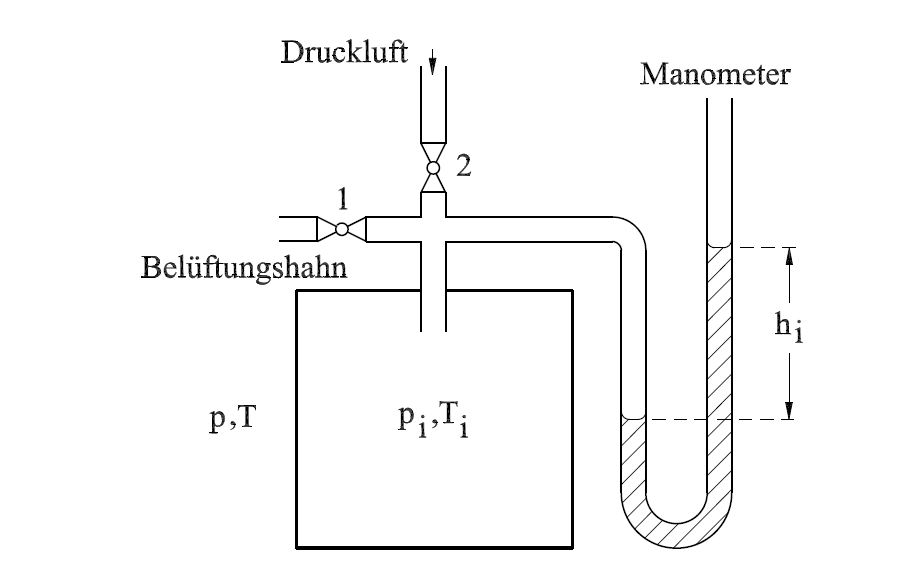
\includegraphics[width=0.8\textwidth]{bilder/aufbau_v2.png}
				\caption{.\cite{WWU}} %TODO Caption
				\label{fig:AufbauV2}	
			\end{figure}
			Abbildung \ref{fig:AufbauV2} stellt den Aufbau graphisch dar.
			Zu erkennen ist ein großes Glasgefäß, welches mit Luft gefüllt ist und der Temperatur $T_i$ und dem Druck $P_i$ unterliegt.
			Dieses Gefäß ist mit einem Manometer verbunden, welches an der rechten oberen Seite offen ist.
			Die beiden Ventile dienen zur Regulierung des Drucks in dem System.
			Bei geschlossenem Ventil 1 lässt sich Druckluft über Ventil 2 in das System einführen und umgekehrt kann der Druck gesenkt werden, wenn die Belüftungsbahn, an Ventil 1, geöffnet wird.
			
		\subsubsection{Funktionsweise}
			
			Entspricht der Druck im Inneren des Systems $P_i$ gerade gleich dem äußeren Luftdruck $P_L$, wie es z. B. bei geöffnetem Ventil 2 der Fall ist, so befindet sich das Manometer in Ruhelage mit einer Höhendifferenz von $h_i = 0$.
			Hierbei ist ebenso $T_i = T_L$, wobei es sich um die Temperatur der Außenluft $T_L$ handelt.
			Ist jedoch $P_i>P_L$, so ist der Flüssigkeitsstand auf der rechten Seite höher als auf der linken.
			Dies führt zu $h_i > 0$.
			Damit auch hier ein adiabatischer Vorgang stattfinden kann, muss der Druck sich schnell genug ändern, dass kein Temperaturausgleich mit der Umgebung möglich ist.
			Dazu wird zunächst der Druck über Ventil 2 erhöht und nach dem Einstellen des Temperaturgleichgewichts in dem System das Ventil 1 mit einer vollständigen Umdrehung geöffnet und wieder geschlossen.
			Dies muss mit der richtigen Geschwindigkeit erfolgen, damit der Druck auf den Außendruck abfallen kann, die Temperatur sich in dem System jedoch nicht ändert.
			
			Seien nun $(P_1,T_1),(P_2,T_2)$ und $(P_3,T_3)$ die Wertepaare direkt nach dem Zuführen der Druckluft (\textrightarrow $T_1 = T_L$ zunächst unverändert), direkt nach dem Temperaturausgleich und dem Drehen von Ventil 1 (\textrightarrow $P_2 = P_L$ auf Außendruck abgefallen), sowie nach dem erneuten Ausgleich der Temperatur (\textrightarrow $T_3 = T_L$ Aufnahme von Wärme aus der Umgebung bis die Temperatur gleich der Außentemperatur ist).
			Dann gilt für den Druck $P_i$ in dem System:
			\begin{equation}
				P_i = P_L + \rho\cdot g\cdot h_i,
			\end{equation} 
			wobei $\rho$ die Dichte der Luft ist.
			Aus dem konstanten Quotient $p/T$ folgt für den isochoren Prozess damit und einigen weiteren Äquivalenzschritten der Adiabatenexponent $\kappa$:
			\begin{equation} \label{eq:kappav2}
				\kappa = \frac{h_1}{h_1-h_3},
			\end{equation}
			dabei ist $h_1$ die Höhendifferenz, die sich nach dem ersten Temperaturausgleich und vor dem Öffnen von Ventil 1 einstellt und $h_3$ nach dem zweiten Temperaturausgleich.
			
	\subsection{Durchführung}
		
		Die Durchführung dieses Teilversuches bestand im Wesentlichen aus dem Notieren der Höhendifferenzen, die sich nach den Temperaturausgleichen nach dem Einführen von Druckluft über Ventil 2 bzw. nach dem kurzen Öffnen von Ventil 1 eingestellt haben.
		Da die richtige Drehgeschwindigkeit für die ersten Messungen nicht getroffen wurde, fand kein Ausgleich von Innen- mit Außendruck statt.
		Dies führte zu Ergebnissen, bei denen $\kappa$ zwischen 2 und 3 lag.
		Aus Zeitgründen wurden statt fünf Messungen jeweils drei Messungen an zwei mal dem gleichen Aufbau durchgeführt.
		Dabei unterscheiden sich nur die abgelesenen Werte für den Stand am Manometer für $h_i = 0$.
		Aus doppelten Abstand von dem Stand auf der rechten Seite dazu wurden dann $h_1$ und $h_3$ bestimmt.
		 
	\subsection{Datenanalyse}
		
		Aus den sechs relevanten Messungen ließ sich $\kappa$ über Gleichung \ref{eq:kappav2} einfach bestimmen.
		Der über die Messungen gemittelte Wert entspricht: $\kappa = $. %TODO Wert
		Wie in dem ersten Teilversuch lässt sich auch hier der Freiheitsgrad von Luft über das berechnete $\kappa$ bestimmen.
		Über Gleichung \ref{eq:Freiheit} folgt hier: $f = $.
		
	\subsection{Diskussion}
		
		Auch hier stellt sich nun die Frage, ob die Ziele der Untersuchung erreicht wurden.
		Wird zunächst der Freiheitsgrad $f = $ betrachtet, so stimmt dieser mit der Anzahl der Freiheitsgraden für zweiatomige Gase, von fünf bis sieben, überein. 
		Drei für Translation, zwei für Rotation und zwei optionale Freiheitsgrade für Schwingung.
		Bei Luft handelt es sich zum größten Teil aus $N_2$ und $O_2$, bei denen es sich um zweiatomige Gase handelt.
		% TODO passt
		 